\documentclass[11pt,aspectratio=169]{beamer}
\usepackage[T1]{fontenc}
\usepackage[utf8]{inputenc}
\usepackage{lmodern}
\usepackage{booktabs,tabularx}
\usepackage{graphicx}
\usepackage{amsmath, amssymb, amsfonts, amsthm, bbm}
\usepackage[
    natbib=true,
    bibencoding=inputenc,
    bibstyle=authoryear-ibid,
    citestyle=authoryear-comp,
    maxcitenames=3,
    maxbibnames=10,
    useprefix=false,
    sortcites=true,
    backend=bibtex
]{biblatex}
\AtBeginDocument{\toggletrue{blx@useprefix}}
\AtBeginBibliography{\togglefalse{blx@useprefix}}
\setlength{\bibitemsep}{1.5ex}
\addbibresource{References.bib}

\usepackage{hyperref}
\hypersetup{
    colorlinks=true,
    linkcolor=black,
    anchorcolor=black,
    citecolor=black,
    filecolor=black,
    menucolor=black,
    runcolor=black,
    urlcolor=black}

\DeclareMathOperator{\argmax}{arg\,max}

%Theorem
\newtheorem{assumption}{Assumption}
\newtheorem{proposition}{Proposition}
%\newtheorem{definition}{Definition}


\begin{document}
\mode<presentation>{	
    \setbeamertemplate{navigation symbols}{}
}

\title{Topics in Behavioral Decisons in Finance}
\date{Discussion by Christian Hilpert\\ \today}
\begin{frame}
    \titlepage
\end{frame}


\begin{frame}{Topics in Behavioral Decisons in Finance}
    \begin{enumerate}
        \item Organisation \\
        \item Brief Overview of Behavioral Economy\\
        \item Comulative Prospect Theory\\
        \item Application and Dimits of CPT \\
        \item Alternative Theories\\
    \end{enumerate}
    $\Rightarrow$ Why?
\end{frame}

\begin{frame}
    \begin{itemize}
        \item Barberis 2017, AEA  \medskip
        \item Thalw 2016, AER \medskip
        \item Barberis 2013, JEP
        \item Wakker 2010, Cambridge University Press, "Prospect Theory for Risk and Ambiguity"
	\end{itemize}
\end{frame}

\begin{frame}{2.Brief Overview}
    1950s-1990s:"Traditional Finance" 
\begin{itemize}
	\item psychological shortcomings \medskip
    \item new way of thinking about Finance questions\medskip
        \begin{enumerate}
            \item  insurance
            \item portfolio choice
            \item corporate finance 
        \end{enumerate}
        \ldots
    \item not alternative to mainstream economics (Micro) \medskip
\end{itemize}
\end{frame}

\begin{frame}{2.Brief Overview}
 Some questions:
    \begin{itemize}
        \item Why do people buy insurance, gamble, and hold stocks?\medskip
        \item Why do people hold on to losing stocks?
        \item Why are IPOs underpriced?
    \end{itemize}
Standard paradigm:
    \begin{itemize}
        \item $t= 0,1,2,...$ time
        \item $S_t$ possible states
        \item $p(s_t)$ probility of $s_t \in S_t$ occuring in $t$
        \item $X_t$ payoff/ consumption in $t$
    \end{itemize}
\end{frame}


\begin{frame}{2.Brief Overview}
\begin{itemize}
    \item Agent-utility function $U(X\mid S)$ \\
\quad - time-independent discount factor $\delta $\\
(implicitily: von-Neumann/Morgenstern axioms)\\
\hspace*{\fill} \\
    \item $\Rightarrow$ max  expected lifetime utility\\
$ \mathop{\max}\limits_{x_t} \mathop{\Sigma}\limits_{t}  \delta^t (\mathop{\sum}\limits_{s_t \in S_t} U(x_t \mid s_t)\rho (s_t)) $\qquad s.t. $x_t \in X_t $\\
\hspace*{\fill} \\
    \item Behavioral Decisions:
    \begin{enumerate}[1.)]
        \item Non-standard preferences : "$U$ ","$\delta $"
        \item Non-standard beliefs: "$\rho$"
        \item Non-standard decision making : "max"
    \end{enumerate}
\end{itemize}
\end{frame}

\begin{frame}{2.Brief Overview}
    \begin{enumerate}[1:]
        \item Reference-dependence, prospect theory, ambiguity\\
        Implies: loss aversion, time preferences (non-standard), self-control issues, time inconsistency, social preferences\\
        \item Overconfidence, extrapolation, experience effects\\
        Implies: overestimation, confirmation bias, projection bias, law of small numbers.\\
        \item Bounded rationality, cognitive limitations.\\
        Implies: rules of thumb??? , simplification, fruniing????(there are ??)
    \end{enumerate}

    Not simply oeparated 1 weakest, 3 strongest depf??  from EU 
\end{frame}

\begin{frame}{2.Brief Overview}
Alternatives:
    \begin{itemize}
        \item Bounded rationality
        \item Evolutionary game theory
        \item Decision theory (unawareness, unforseen contingencies)
    \end{itemize}
Behavioral economics is controversial!
    \begin{itemize}
        \item poor experimental standards
        \item depo?? from revealed preference approaches
    \end{itemize}    
\end{frame}

\begin{frame}{3.Prospect Theory and Cumulative PT}
    \begin{itemize}
        \item most finance models assume EU to evaluate risks
        \item experimentally, at least, not a good fit
        \item many alternatives 
        \item (C)PT by Kahneman and Tversky 1979, Tversky and Kahneman1992\\
        \item alternatives: disappointment aversion, rank-dependent utility, salume theory, regeret theory, SP8H Hec???
    \end{itemize} 
\end{frame}


\begin{frame}{3.Prospect Theory and Cumulative PT}
    \begin{itemize}
        \item A reference-dependent utility function is a family\\
    $ \{U(\cdot \mid \gamma):x \longrightarrow \mathbb{R} \mid \gamma \in X\} $ 
    of utility functions over $X$ indexed by $\gamma \in X$.\\
        \item the utility $U(X \mid \gamma)$ describes the utility of the consumption and the reference point is $\gamma$.\\
\hspace*{\fill} \\
        \item Prospect Theory (1979)\\
            gramble $ (X,p,y,q)$\\
            $EU=p V(w +x)+qV(w+y)$\\
            $PT=w(p)V(x)+w(q)V(y)$\\
\end{itemize}  
\end{frame}
\begin{frame}
    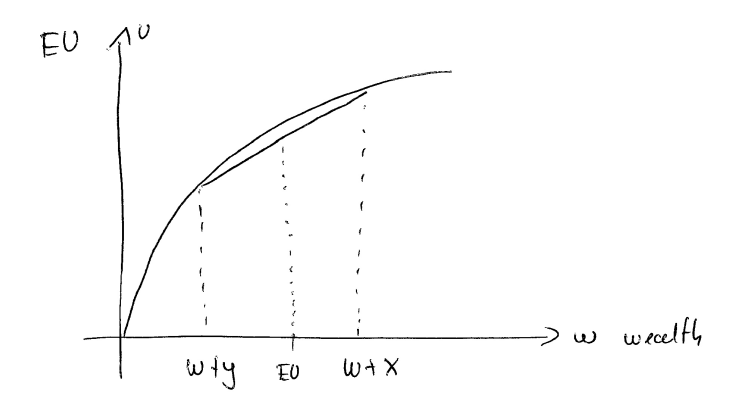
\includegraphics[width = 0.5\textwidth]{fig1.png}
    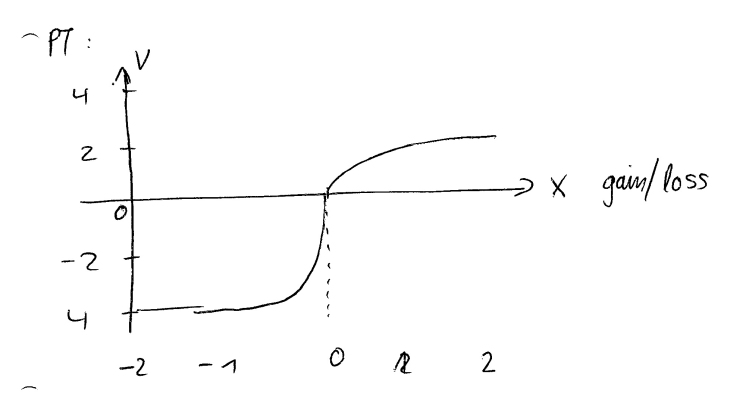
\includegraphics[width = 0.4\textwidth]{fig2.png}
	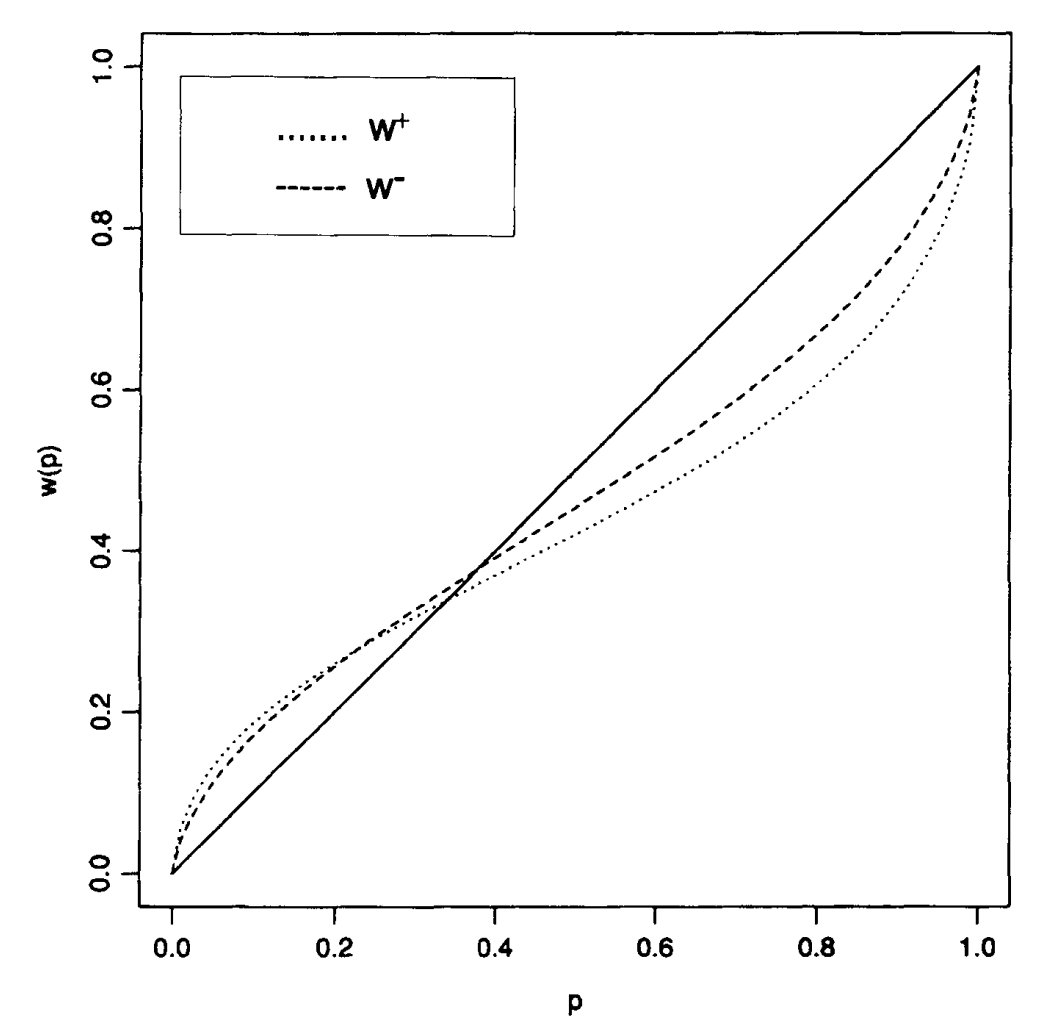
\includegraphics[width = 0.4\textwidth]{fig3.png}
\end{frame}

\begin{frame}{Four key features}
    \begin{enumerate}[1.]
        \item Reference-dependence
            \begin{itemize}
                \item gains and losses, and final wealth
                \item $\Rightarrow$ experimental evidence, consistent with perception of alternative \medskip
            \end{itemize}
        \item Loss aversion
            \begin{itemize}
                \item $V(x)$ has a kink?? in $\bigcirc$ .
                \item $\Rightarrow$ losses loom larger than gains.\\
                \item   evidence: $(110,\frac{1}{2},-100,\frac{1}{2})$ is unatterative.
            \end{itemize}
    \end{enumerate}
\end{frame}

\begin{frame}{Four key features}
    \begin{enumerate}[3.]
        \item Dimisishing sensitivity\\
            \begin{itemize}
                \item $V(\cdot)$ concave over gains, convex over losses
                \item evidence: $(500,1) \succ (1000,\frac{1}{2})$\\
                \qquad  $(-500,1) \preceq  (-1000,\frac{1}{2})$
            \end{itemize}
            \hspace*{\fill} \\
    \end{enumerate}
    \begin{enumerate}[4.]
        \item Probability weighting:\\
            \begin{itemize}
                \item transform probability with decision weights $w(\cdot )$\\
                high weight on low probabilities\\
                \item evidence: $(5,1)\prec (5000,0.001)$ lottery\\
                \qquad  $(-5,1)\succ (-5000,0.001)$ insurance
            \end{itemize}
            Note: $w$ are decision weights and beliefs
    \end{enumerate}
\end{frame}

\begin{frame}{Cumulative Prospect Theory (Tversky and Kahneman,1992)}
    \begin{itemize}
        \item address some limitations\\
        \item applies probability weighing to the comulative distribution function \medskip
        (gain at least 50, lose 100 or more)\\
        $(x_{-m},p_{-m},...,x_{-1},p_{-1},x_0,p_0,x_1,p_1,...,x_n,p_n)$ \\
        $x_i < x_j$ for $i<j,x_0=0$ \\
        is assigned \qquad
        $ \sum_{i=-m}^{n} \pi_i V(x_i)$\\
        with\\
            \begin{equation}
                \pi_i = \begin{cases}
                w(p_i+...+p_n) - w(p_i+...+p_n),  & 0\leq i \leq  n\\
                w(p_{-m}+...+p_i) - w(p_{-m}+...+p_{i-1}),  & -m\leq i \leq 0\\
            \end{cases}
            \end{equation}\medskip
        \item individuals overweight fails of a probability distribution\\
        \item preserves a taste for lottery like gambles
    \end{itemize}
\end{frame}

\begin{frame}{Cumulative Prospect Theory (Tversky and Kahneman,1992)}
    \begin{itemize}
        \item Tversky and Kahneman suggest:\\
    \end{itemize}
    \hspace*{\fill} \\
\begin{equation}
    V(x) = \begin{cases}
    x^\alpha,  & x\geq 0\\
    -\lambda (-x)^\alpha,  & x< 0\\
    \end{cases}
\end{equation}\medskip
\centering $ w(p) = \frac{p^{\delta}}{(p^{\delta}+(1-p)^{\delta})^{\frac{1}{\delta}}} $\\
$\alpha =0.88 ,\quad \lambda =2.25, \quad \delta =0.69 $ ??? \\
\hspace*{\fill} \\
\begin{itemize}
    \item (there are alternatives)\\
\end{itemize}
\end{frame}

\begin{frame}{Challenges and Discussion}
    \begin{itemize}
        \item how to define gains and losses?\\
        \item total wealth, financial wealth, stock holdings, individual stocks?\\
        \item what is a gain:\\
        \begin{itemize}
            \item exceeds zero?\\
            \item risk-free rate?\\
            \item expectation?\\
        \end{itemize}
        \item probability weighting in many applications more important than loss aversion\\
        \item diminishing sensitivity  $\Rightarrow$  Rabin $2000$ \\
        (not as important feature theoretically)
        \item overweighting VS underweighting:??? events\\
        (Taleb ,2007),evidence for both\\
        \item could be \\
        \qquad decision from description $\Rightarrow$ overweighting\\
        \qquad decision from experience $\Rightarrow$ underweighting\\
        \item not ?? decv how to interpret:
        \qquad overestimation (belief) $\Rightarrow$ mistake\\
        \qquad overweighting (preference) $\Rightarrow$ not mistake???\\
        (some evidence fro preference)
    \end{itemize}  
\end{frame}

\end{document}
